\chapter{Discussion}
\textbf{Stikord}
\begin{enumerate}
    \item If we had chosen another model, the conclusion from the cross-validation and f-test might have been different.
    \item Section 3.2.1 -> There exists estimator that are better than least squares but are biased, maybe it would be better to use a biased estimator with lower variance. The Bias-Variance trade-off. 
    \item Sammenlign med hvis vi havde lavet $k=n$ fold i cv.
    \item Prediction interval stort
    \item Diskutere hvordan vi kunne have delt condition op til dårlig og ok/god istedet.
    \item Vores før krise, krise og efter krise vriabel smider en masse information ud, når vi anvender den for 2016. Derfor er vores predictions så dårlige, da vi ser på efter krisen som et gennemsnit af 12-15 dataen. Men da det går meget bedre i 2016 for huspriserne end nogle af de andre år i denne kategori, da underpredikter vi alt vores data for 2016. (VIGTIG) Fy esben fy!! Plot residualer mod årstal og konkluder systematik. Snakke om at der er stor variation i vores indeling af tidsperioderne. Så vægtet gennemsnit giver store residualer. 
\end{enumerate}

\begin{figure}[H]
        \centering
      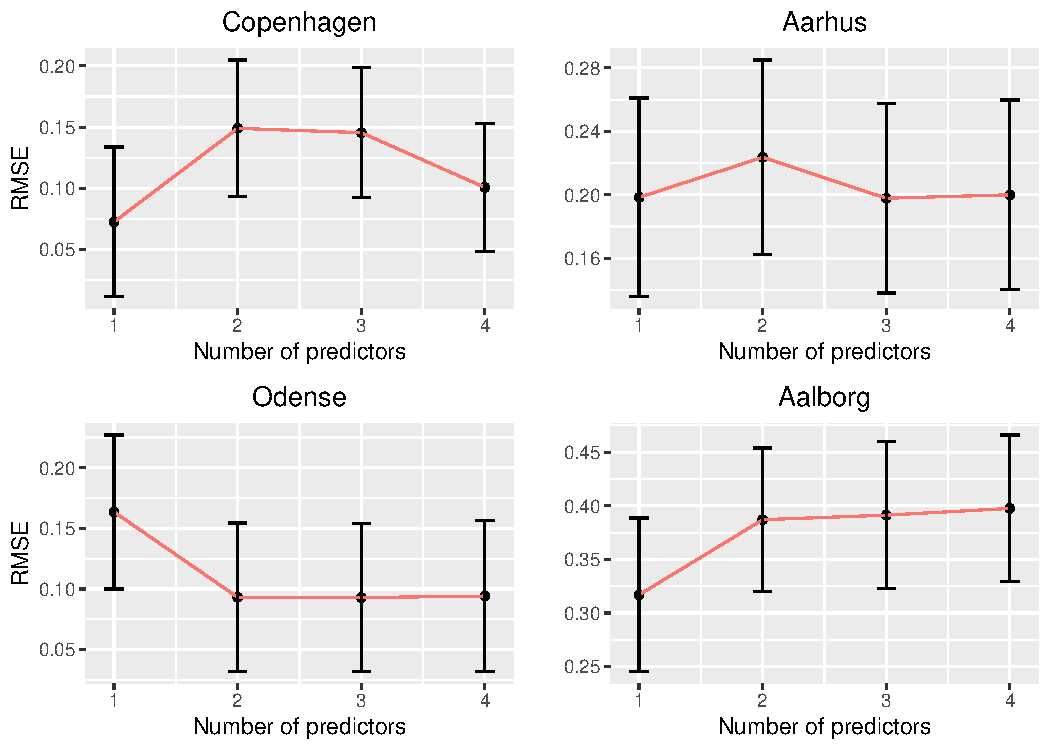
\includegraphics[width = 0.7 \textwidth]{figures/Nanna/k=n.pdf}
      \caption{Result from $k = n$ fold cross-validation.}
      \label{fig:error_cont}
\end{figure}



Section 3.2.1 -> There exists estimator that are better than least squares but are biased, maybe it would be better to use a biased estimator with lower variance. The Bias-Variance trade-off. 